\documentclass[12pt,a4paper,portrait]{article}

\usepackage[portuguese]{babel} 	% hifenização
\usepackage[utf8]{inputenc} 	% acentos e cedilhas
\usepackage[T1]{fontenc} 		% evitar problemas com fonts
\usepackage{graphicx}
\usepackage{graphicx,wrapfig}
\usepackage{fancyhdr}
\usepackage{lastpage}
\usepackage[dvipsnames]{xcolor}
\usepackage{colortbl}
\usepackage{enumerate}			% Include the enumerate-package
\usepackage{listings}           % Include the listings-package
\usepackage{color}				% Include the color-package
\usepackage{askmaps}
\usepackage{booktabs}
\usepackage{xcolor}

\usepackage{babel}
\usepackage[font=small,labelfont=bf]{caption}

\pagestyle{fancy}
\fancyhf{}
\rhead{Engenharia Informática 2º Ano}
\lhead{ISMAT}
\rfoot{Página \thepage \hspace{1pt} de \pageref{LastPage}}

\setcounter{secnumdepth}{5}	% actualiza o contador máximo de níveis para subsections
\setcounter{tocdepth}{5}	% actualiza o contador máximo de níveis na Tabela de Conteudo

\begin{document}
	\begin{titlepage}
	\begin{center}
	
		% Upper part of the page. The '~' is needed because \\
		% only works if a paragraph has started.
		%
\includegraphics[width=0.95\textwidth]{./logo}~\\[1,5cm]
		
\includegraphics{./logo}
		% \includegraphics{logo_ismat}
		
		
		%\textsc{\LARGE Instituto Superior Manuel Teixeira Gomes }\\[1.5cm]
		
		\textsc{\Large Algoritmia e Estrutura de Dados}\\[1.5cm]
		
		% Title
		\newcommand{\HRule}{\rule{\linewidth}{0.5mm}}
		\HRule \\[0.4cm]
		{ \huge \bfseries Travel Salesman Problem \\[0.4cm] }
		
		\HRule \\[1.5cm]
		
		% discente e docente
		\noindent
		
		\begin{minipage}[t]{0.4\textwidth}
			\begin{flushleft} \large
				\emph{Discente(s):}\\
				Pedro \textsc{Roldan}\\
				Leandro \textsc{Moreira}\\
			\end{flushleft}
		\end{minipage}%
		\begin{minipage}[t]{0.4\textwidth}
			\begin{flushright} \large
				\emph{Docente:} \\
				Doutor Faroq \textsc{AlTam}
			\end{flushright}
		\end{minipage}
		
		\vfill
		
		% Bottom of the page
		{\large \today}
	
	\end{center}
\end{titlepage}
	\tableofcontents
	
	\lstdefinestyle{customc}{
	  belowcaptionskip=1\baselineskip,
	  breaklines=true,
	  frame=L,
	  xleftmargin=\parindent,
	  language=C,
	  showstringspaces=false,
	  basicstyle=\footnotesize\ttfamily,
	  keywordstyle=\bfseries\color{green!40!black},
	  commentstyle=\itshape\color{purple!40!black},
	  identifierstyle=\color{blue},
	  stringstyle=\color{orange},
      tabsize=1,
	}
	
	\newpage
	\section{Introdução}
		O travel salesman problem (TSP) é um problema bastante comum largamente encontrado em diversas aplicações tais como: empresas de transporte (e.g. UPS), escalas de tripulação de companhias aéreas, etc.\\
		Em principio, um vendedor necessita de efetuar uma viagem por diversas cidades, onde inicia a viagem numa determinada cidade (Casa), visita todas as cidades para vender os seus produtos, e retorna a casa.\\
		\subsection{Requisitos Minimos}	
			O TSP pode ser representado por uma lista de nós, sendo o objectivo descobrir uma serie de caminhos (Edges) entre cada um dos nós.\\\\
			Sendo que:\\
			\begin{itemize}
				\item Cada nó (Cidade) pode ser visitado apenas 1 vez.
				\item Os caminhos formam uma Tour.
				\item O custo da Tour deve ser o minimo possivel.
			\end{itemize}
			A tour TSP é um grafico direcionado, onde cada nó representa uma cidade, e cada edge representa um caminho entre 2 cidades.\\
			Cada edge têm um peso, que é no seu caso mais simples a distancia euclidiana entre os seus nós.\\
			Este peso pode ser composto por diversos fatores, no entanto neste projeto apenas se considera a distancia entre nós.\\ 			
		\subsection{O circuito main}
			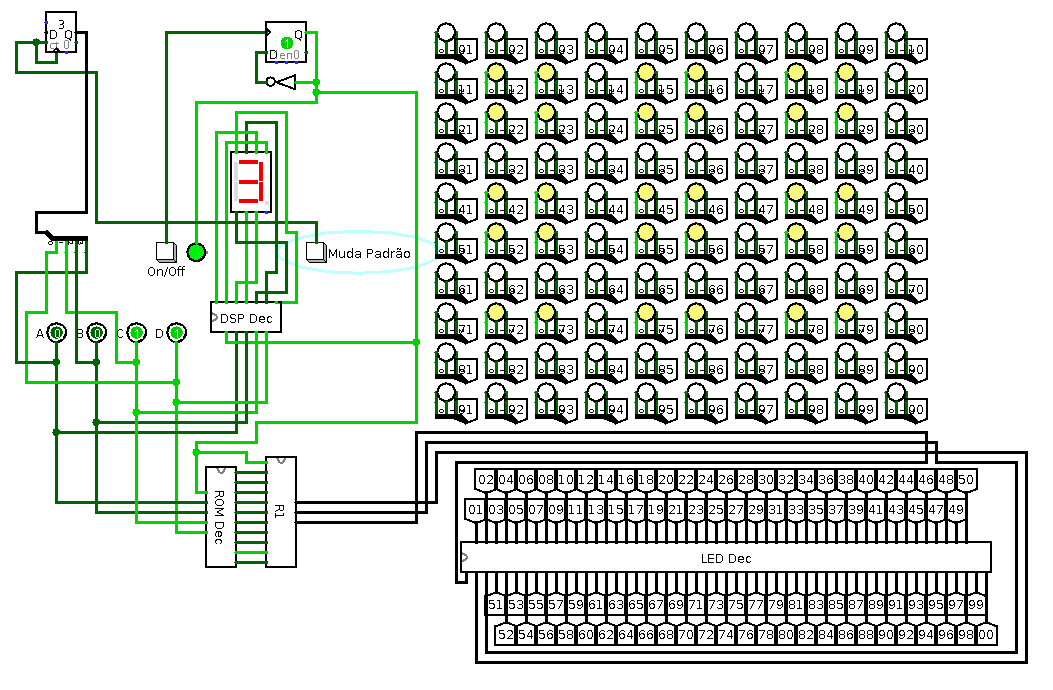
\includegraphics[width=1.0\textwidth]{imagens/main}\\
			Esta é a representação geral do circuito digital.\\
			Conforme podemos observar o circuito encontra-se dividido em 4 circuitos que se interligam de forma a que o sistema funcione como um todo.\\
			\begin{itemize}
				\item Matriz de Leds 10x10 (300 leds).
				\item Controlo Geral (Botão de controlo geral on/off e indicador visual).
				\item Mostrador de padrões do sistema (10 padrões disponíveis).
				\item Circuito com as ROM do sistema.
				\item Circuito de controle da matriz de leds.
			\end{itemize}
			De salientar que existem diversos pontos no circuito que poderiam ser eliminados, existindo apenas para que seja possível a visualização dos seus valores binarios.\\
			\subsubsection{Matriz de leds}
				\begin{minipage}{1.1\textwidth}
					\begin{minipage}[b]{0.49\textwidth}
						A matriz de leds é composta por uma grelha de 10x10, onde em cada posição esta um conjunto de 3 leds, a fim de emular o correto funcionamento de um led RGB.\\
						Temos então uma grelha composta por 300 leds conforme a imagem no seu estado desligado.\\
						Cada grupo de RGB Leds é então endereçável através de um conjunto de bits de controlo, processo que é descrito em \ref{ssec:num1} e \ref{ssec:num2} onde se pode visualizar a implementação realizada no circuito.
					\end{minipage}
					\hfill
					\begin{minipage}[b]{0.49\textwidth}
						\centering
						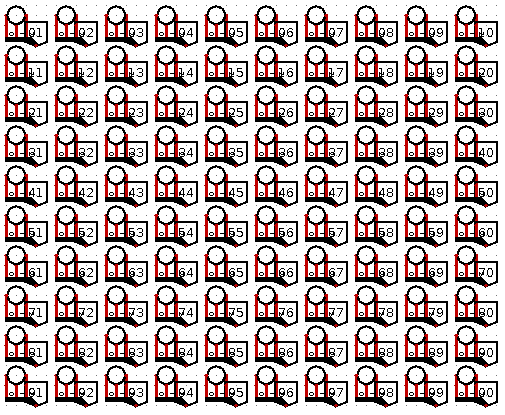
\includegraphics[width=1.0\textwidth]{imagens/ledmatrix}
						\captionof{figure}{Matriz de Leds 10x10}
					\end{minipage}
				\end{minipage}\\
		\subsection{Display de 7 segmentos}
			O display de 7 segmentos é um dispositivo bastante usado para indicação de valores numéricos.\\
			Desde que ele pode indicar dígitos de 0 a 9 (10 dígitos), a informação binária precisa ter 4 dígitos binários, pois, com três, só oito valores podem ser exibidos.\\
			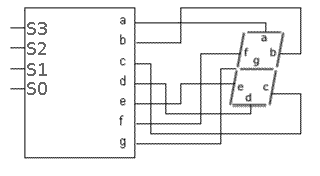
\includegraphics[width=0.5\textwidth]{imagens/7digit}\label{img:7digit}\\
			Neste circuito, S0-S4 são as quatro entradas binárias e Q0-Q6 são as saídas para os sete segmentos do display.\\
			%\clearpage
			\begin{table}[!h]
				\centering
				\caption{Tabela de verdade}
				\label{7digitl}
				\resizebox{0.6\textwidth}{!}{%
					\begin{tabular}{@{}|l|llll|lllllll|@{}}
						\toprule
						\rowcolor[HTML]{BBDAFF} 
						 & D & C & B & A & Q0 & Q1 & Q2 & Q3 & Q4 & Q5 & Q6 \\ \midrule
						0 & 0 & 0 & 0 & 0 & 1 & 1 & 1 & 1 & 1 & 1 & 0 \\
						1 & 0 & 0 & 0 & 1 & 0 & 1 & 1 & 0 & 0 & 0 & 0 \\
						2 & 0 & 0 & 1 & 0 & 1 & 1 & 0 & 1 & 1 & 0 & 1 \\
						3 & 0 & 0 & 1 & 1 & 1 & 1 & 1 & 1 & 0 & 0 & 1 \\
						4 & 0 & 1 & 0 & 0 & 0 & 1 & 1 & 0 & 0 & 1 & 1 \\
						5 & 0 & 1 & 0 & 1 & 1 & 0 & 1 & 1 & 0 & 1 & 1 \\
						6 & 0 & 1 & 1 & 0 & 1 & 0 & 1 & 1 & 1 & 1 & 1 \\
						7 & 0 & 1 & 1 & 1 & 1 & 1 & 1 & 0 & 0 & 0 & 0 \\
						8 & 1 & 0 & 0 & 0 & 1 & 1 & 1 & 1 & 1 & 1 & 1 \\
						9 & 1 & 0 & 0 & 1 & 1 & 1 & 1 & 1 & 0 & 1 & 1 \\
						 & 1 & 0 & 1 & 0 & x & x & x & x & x & x & x \\
						 & 1 & 0 & 1 & 1 & x & x & x & x & x & x & x \\
						 & 1 & 1 & 0 & 0 & x & x & x & x & x & x & x \\
						 & 1 & 1 & 0 & 1 & x & x & x & x & x & x & x \\
						 & 1 & 1 & 1 & 0 & x & x & x & x & x & x & x \\
						 & 1 & 1 & 1 & 1 & x & x & x & x & x & x & x \\ \bottomrule
					\end{tabular}
				}
			\end{table}
			A notação x indica valor indiferente (pode ser 0 ou 1), uma vez que não há valor a exibir acima da combinação 9.\\
			Conforme referido em \ref{sssec:bcd}, a informação binária não tem necessariamente relação com o número binário que ela representa.\\
			Por exemplo, para a combinação 0, Q0 Q1 Q2 Q3 Q4 Q5 Q6 tem 1111110. Este número binário não é igual ao dígito correspondente no display (0).\\
			Isto é, na realidade, um código para o display de 7 segmentos.\\			
			\subsubsection{Mapa Veitch-Karnaugh}
			 A partir da tabela de verdade, temos quatro entradas S0-S4 e 7 saidas Q0-Q6, que são eletricamente independentes, considera-se que cada saída é um circuito e foi elaborado um mapa para cada.\\
			 Obtemos então uma expressão POS simplificada a partir do seu respetivo mapa para cada uma das saídas.\\
			\begin{minipage}{1.1\textwidth}
				\begin{minipage}[b]{0.49\textwidth}
					\centering
					\askmapiv{Q0}{abcd}{}{101x011x11xx11xx}{
					}
					\captionof{table}{Q0=$\overline{S2}$$\overline{S0}$+$S1$+$S2$$S0$+$S3$}
				\end{minipage}
				\hfill
				\begin{minipage}[b]{0.49\textwidth}
					\centering
					\askmapiv{Q1}{abcd}{}{111x101x10xx11xx}{
					}
					\captionof{table}{Q1=$\overline{S2}$+$\overline{S1}$$\overline{S0}$+$S1$$S0$}
				\end{minipage}
			\end{minipage}\\
			\begin{minipage}{1.1\textwidth}
				\begin{minipage}[b]{0.49\textwidth}
					\centering
					\askmapiv{Q2}{abcd}{}{111x101x10xx11xx}{}
					\captionof{table}{Q2=$\overline{S1}$+$S0$+$S2$}
				\end{minipage}
				\hfill
				\begin{minipage}[b]{0.49\textwidth}
					\centering
					\askmapiv{Q3}{abcd}{}{111x101x10xx11xx}{}
					\captionof{table}{Q3=$\overline{S2}$$\overline{S0}$ +$\overline{S2}$$S1$ + $S1$$\overline{S0}$ + $S2$$\overline{S1}$$S0$ +$S3$}
				\end{minipage}
			\end{minipage}\\
			\begin{minipage}{1.1\textwidth}
				\begin{minipage}[b]{0.49\textwidth}
					\centering
					\askmapiv{Q4}{abcd}{}{111x101x10xx11xx}{}\\
					\captionof{table}{Q4=$\overline{S2}$$\overline{S0}$+$S1$$\overline{S0}$}
				\end{minipage}
				\hfill
				\begin{minipage}[b]{0.49\textwidth}
					\centering
					\askmapiv{Q5}{abcd}{}{111x101x10xx11xx}{}
					\captionof{table}{Q5=$\overline{S1}$$\overline{S0}$+$S2$$\overline{S1}$+$S2$ $\overline{S0}$+$S3$}
				\end{minipage}
			\end{minipage}\\
			\begin{minipage}{1.1\textwidth}
				\begin{minipage}[b]{0.49\textwidth}
					\centering
					\askmapiv{Q6}{abcd}{}{111x101x10xx11xx}{}\\
					\captionof{table}{Q6=$\overline{S2}$${S1}$+$S2$$\overline{S1}$+$S2$ $\overline{S0}$+$S3$}
				\end{minipage}
				\hfill
				\begin{minipage}[b]{0.49\textwidth}
				\end{minipage}
			\end{minipage}\\\\									
			Os valores indiferentes (X) devem ser inseridos. Como podem ser 0 ou 1, supõem-se valores convenientes para formar grupos os maiores possíveis.Quanto maior o grupo, menor o número de variáveis e o circuito é mais simples.\\
		\subsubsection{DSP Decoder} \label{ssec:num2}
			De forma a que fosse possível implementar um display de 7 segmentos foi necessário efetuar diversas operações, de forma a obter o resultado implementado que mostra os 10 padrões disponíveis no sistema.\\\\
			Tendo a expressão simplificada para cada uma das saídas Q0-Q7, podemos então implementar o respetivo circuito de forma a que cada digito binário recebido tenha a sua correspondência em \textbf{código BCD} na saída.\\\\
			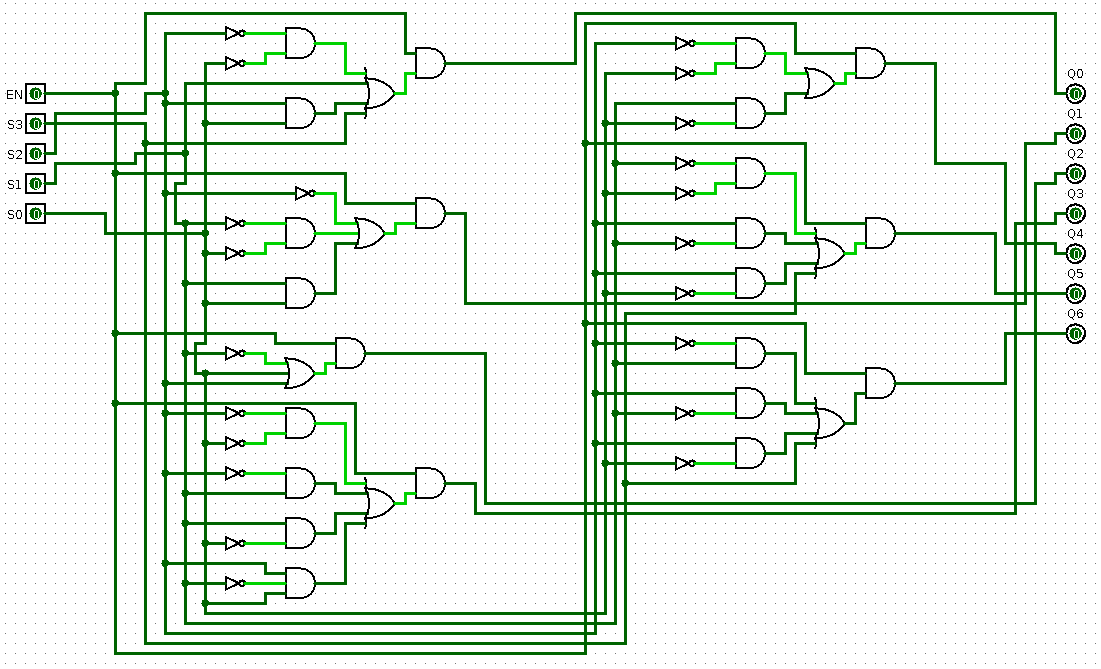
\includegraphics[width=1.0\textwidth]{imagens/dspdec}\\
			\captionof{figure}{DSP Decoder}
			EN: Bit de controlo enable/disable\\
			S0-S3: Conjunto binário de 4 bits correspondendo ao seu valor decimal\\
			Q0-Q7: Conjunto binário para ligação ao display 7-segmentos conforme indicado em \ref{img:7digit}.\\\\
			
			\begin{minipage}{1.1\textwidth}
				\begin{minipage}[b]{0.49\textwidth}
					De forma a exemplificar o valor $7_{10}$ tem a sua correspondência ao binário $0111_{BCD}$\\
				\end{minipage}
				\hfill
				\begin{minipage}[b]{0.49\textwidth}
					\centering
					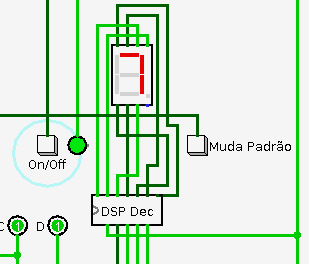
\includegraphics[width=0.7\textwidth]{imagens/7dispon}
					\captionof{figure}{Display 7-Segmentos}
				\end{minipage}
			\end{minipage}\\
		\subsection{LED Decoder}
			Este é o circuito que controla a matriz de leds.\\
			Contendo 3 entradas, recebe em S0 um conjunto de 3 bits que definem a cor do led, em S1 e S2, recebem um conjunto de 10 bits que definem as linhas e as colunas respetivamente, indicando o led a ser usado na grelha.\\\\		
			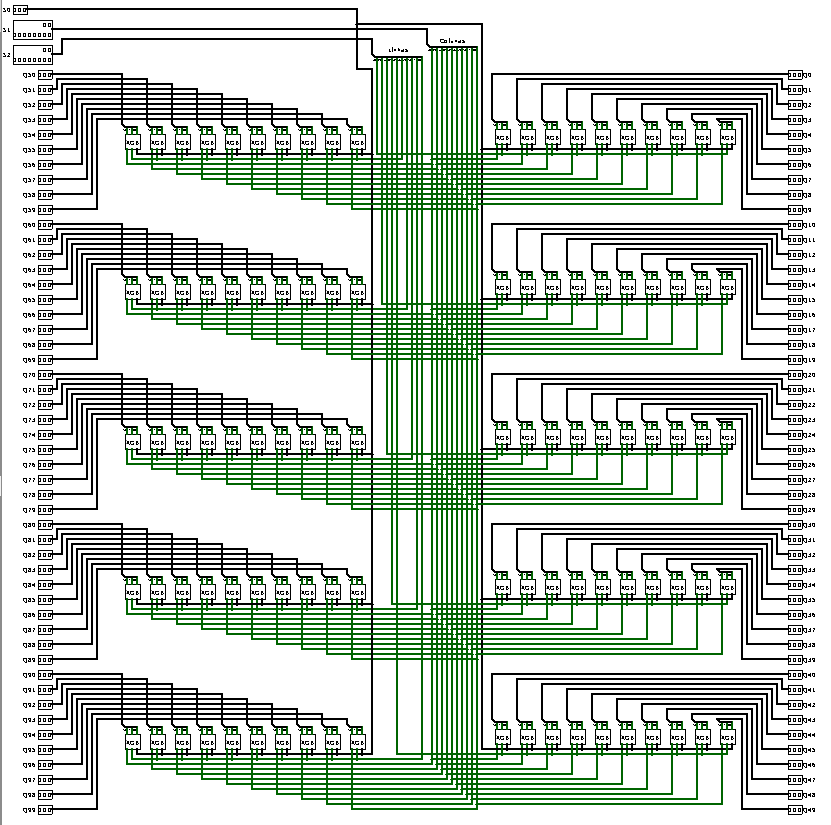
\includegraphics[width=1.0\textwidth]{imagens/leddec}\\
			\captionof{figure}{Circuito LED Decoder}
			S0-S3: Conjunto binário de 4 bits correspondendo ao seu valor decimal\\
			Q0-Q99: Conjunto  de saída para ligação ao led RGB\\
			\newpage
			\subsubsection{RGB Decoder} \label{ssec:num1}
				A função deste circuito é a de ao receber a indicação de posição através do grupo binário de S0 e S1, efetuar a correspondência de cor para a saída do led correspondente, através da separação do grupo de 3 bits.\\
				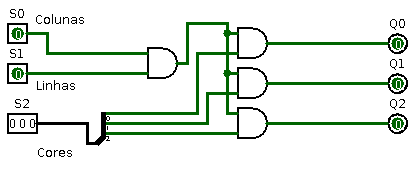
\includegraphics[width=1.0\textwidth]{imagens/rgbdec}
				\captionof{figure}{RGB Decoder}
				S0-S3: Conjunto binário de 4 bits correspondendo ao seu valor decimal\\
		\newpage						
		\subsection{ROM}
			A ROM (read-only memory), é um tipo de memória que permite apenas a leitura, ou seja, as suas informações são gravadas uma única vez e após isso não podem ser alteradas ou apagadas, somente acedidas. São memórias cujo conteúdo é gravado permanentemente.\\\\
			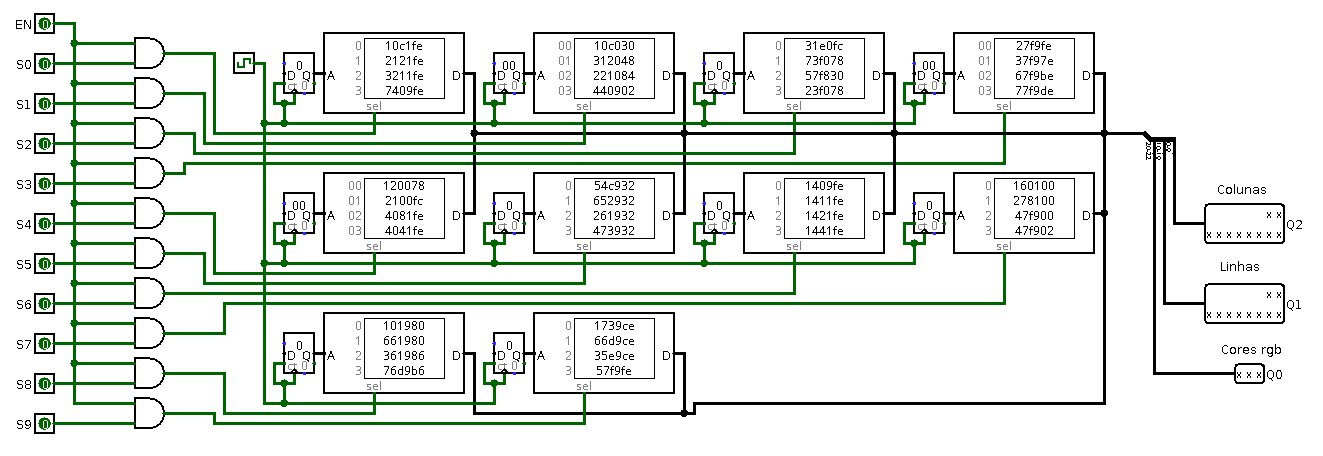
\includegraphics[width=1.0\textwidth]{imagens/romr1}
			\captionof{figure}{Circuito de controle de ROMS}
			EN: Bit de controlo de enable/disable\\
			S0-S9: Bit de entrada para seleção de ROM\\
			Q0: Conjunto de 3 bits para seleção de cor RGB\\
			Cada ROM é controlada por um contador exclusivo e um clock partilhado.\\
			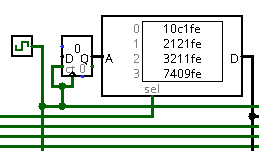
\includegraphics[width=0.5\textwidth]{imagens/rom1}
			\captionof{figure}{ROM Individual}
			Cada ROM tem uma estrutura dimensionada para cada conjunto de sequencias ..\\
			A ROM é controlada por um contador associado a um clock, que permite que, em cada ciclo o contador avançe para uma nova posição (index) da ROM e efetue a leitura da sequencia de bits armazenada, que por sua vez define o endereço do led na matriz, assim como a sua cor e estado.\\
			\subsubsection{BCD - Binary Coded Decimal} \label{sssec:bcd}
				O \cite{Garroz}\textbf{código BCD} foi criado para codificar os números decimais de 0 a 9, com 4 bits para cada dígito, ou seja, o BCD é a conversão dos decimais em um número binário de 4 bits e representa-se da seguinte forma:
				\begin{table}[!h]
					\centering
					\caption{Tabela BCD}
					\label{my-label}
					\resizebox{0.5\textwidth}{!}{%
						\begin{tabular}{@{}|l|l|@{}}
							\toprule
							\rowcolor[HTML]{BBDAFF} 
							Digito Decimal & Codigo BCD \\ \midrule
							0 & 0000 \\ \midrule
							1 & 0001 \\ \midrule
							2 & 0010 \\ \midrule
							3 & 0011 \\ \midrule
							4 & 0100 \\ \midrule
							5 & 0101 \\ \midrule
							6 & 0110 \\ \midrule
							7 & 0111 \\ \midrule
							8 & 1000 \\ \midrule
							9 & 1001 \\ \bottomrule
						\end{tabular}%
					}
				\end{table}\\
				Desta forma foi realizada a codificação segundo cada palavra do código BCD, que corresponde ao digito decimal correspondente a cada ROM utilizada.\\
			\subsubsection{ROM Decoder}
				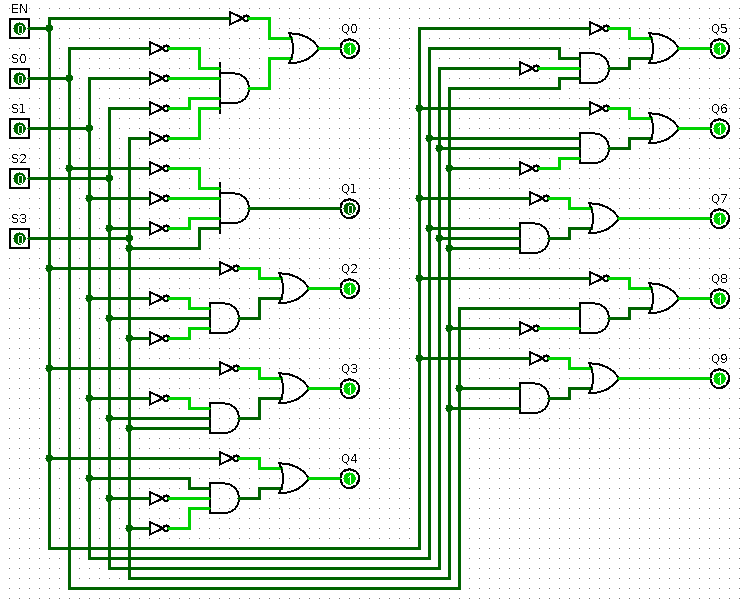
\includegraphics[width=1.0\textwidth]{imagens/romdec}
				\captionof{figure}{Circuito ROM Decoder}			
				EN: Bit de controlo de enable/disable\\
				S0-S3: Conjunto de 4 bits de entra que determina a escolha da ROM a ser utilizada\\
				Q0-Q9: Bit de controlo de saída com escolha de ROM \\
				\begin{table}[!ht]
					\centering
					\caption{Tabela de Seleção de ROM}
					\label{romd}
					\resizebox{0.7\textwidth}{!}{%
						\begin{tabular}{@{}|l|llll|llllllllll|@{}}
							\toprule
							\rowcolor[HTML]{BBDAFF} 
							& S3 & S2 & S1 & S0 & Q0 & Q1 & Q2 & Q3 & Q4 & Q5 & Q6 & Q7 & Q8 & Q9\\ \midrule
							0 & 0 & 0 & 0 & 0 & 1 & 0 & 0 & 0 & 0 & 0 & 0 & 0 & 0 & 0\\
							1 & 0 & 0 & 0 & 1 & 0 & 1 & 0 & 0 & 0 & 0 & 0 & 0 & 0 & 0\\
							2 & 0 & 0 & 1 & 0 & 0 & 0 & 1 & 0 & 0 & 0 & 0 & 0 & 0 & 0\\
							3 & 0 & 0 & 1 & 1 & 0 & 0 & 0 & 1 & 0 & 0 & 0 & 0 & 0 & 0\\
							4 & 0 & 1 & 0 & 0 & 0 & 0 & 0 & 0 & 1 & 0 & 0 & 0 & 0 & 0\\
							5 & 0 & 1 & 0 & 1 & 0 & 0 & 0 & 0 & 0 & 1 & 0 & 0 & 0 & 0\\
							6 & 0 & 1 & 1 & 0 & 0 & 0 & 0 & 0 & 0 & 0 & 1 & 0 & 0 & 0\\
							7 & 0 & 1 & 1 & 1 & 0 & 0 & 0 & 0 & 0 & 0 & 0 & 1 & 0 & 0\\
							8 & 1 & 0 & 0 & 0 & 0 & 0 & 0 & 0 & 0 & 0 & 0 & 0 & 1 & 0\\
							9 & 1 & 0 & 0 & 1 & 0 & 0 & 0 & 0 & 0 & 0 & 0 & 0 & 0 & 1\\ \bottomrule
						\end{tabular}
					}
				\end{table}\\
	\section{Enquadramento}
	O trabalho descrito neste relatório foi realizado recorrendo à linguagem de programação C, assim como os recursos disponibilizados na unidade curricular.\\
		\subsection{Motivação}
			A principal motivação para a realização deste trabalho, resulta da importância em criar e otimizar um sistema digital, assim como demonstrar os conhecimentos alcançados na disciplina de sistemas digitais.\\
		\subsection{Objectivos}
			Pretende-se através deste trabalho, criar um sistema de luzes como \cite{Csoares}Sistema Digital que implementa um sistema de luzes de acordo com um ou mais padrões.\\		
			Em ultima analise o sistema digital é um sistema eletrónico onde os níveis de tensão elétrica são  mapeados como “0” e “1”.\\
			Na saída do circuito encontram-se ligados LEDs que estarão acesos ou apagados com “1” ou “0”, respetivamente.\\
	\section{Conclusões}
		A matriz de leds desenvolvida, para além de permitir os requisitos pedidos no enunciado do trabalho prático, permite também o uso de animações com leds mais complexas, mais padrões disponíveis e sendo modular torna-se mais escalável, entre outras funcionalidades.\\
		De frisar que devido à liberdade proporcionada para a construção dos circuitos, quer na sua forma de desenvolvimento quer na implementação permitiu desta forma aguçar a curiosidade para o uso de diversos componentes do simulador Logisim.\\
		Foi sem duvida um desafio interessante, mas que por limitação de tempo, deixa ainda uma larga margem para melhoramentos.\\
	\newpage
	\section{Bibliografia}
	\bibliographystyle{plain}
	\bibliography{./bibliotecas}

	\newpage
	\section{Anexos}
		Ficheiro "relatorio.pdf" e "ledmatrix.circ" compactado num ficheiro "trabalho.zip".\\\\
		Não existem quaisquer códigos ou listagens adicionais.\\					
\end{document}          
